\documentclass[12pt, a4paper, twoside, openright]{Thesis} % Paper size, default font size and one-sided paper
\usepackage[utf8]{inputenc}
\usepackage{wrapfig}
\usepackage{lscape}
\usepackage{rotating}
\usepackage{graphicx}
\usepackage{caption}
\usepackage{amsmath, nccmath}
\usepackage{comment}
\usepackage{afterpage}
\usepackage{multirow}
\usepackage{multicol}
\usepackage{cleveref}
\usepackage{rotating}
% \usepackage[font=small]{caption}
% \captionsetup{compatibility=false}
% \usepackage{subcaption}
% \usepackage{subfig}
\usepackage{makecell}
\usepackage{booktabs}
\usepackage{multirow}
\usepackage{lscape}
\usepackage{longtable}
\usepackage{placeins}
\usepackage{adjustbox}
\usepackage{arydshln} % dashed midline
\usepackage{ragged2e}
\usepackage{lipsum}
\usepackage{mathtools} % To use box inside an aligned environment
\usepackage{enumitem} % for roman letter lists
% \usepackage{subfig}
\newcommand\myemptypage{
    \null
    \thispagestyle{empty}
    \addtocounter{page}{-1}
    \newpage
    }
%\usepackage[width=14cm, left=3cm]{geometry}

% prints author names as small caps


%\usepackage{subcaption} %incompatible with subfig
\graphicspath{{Pictures/}} % Specifies the directory where pictures are stored
\usepackage[authoryear]{natbib}
%\usepackage[square, numbers]{natbib} % Use the natbib reference package - read up on this to edit the reference style; if you want text (e.g. Smith et al., 2012) for the in-text references (instead of numbers), remove 'numbers' v
%\bibliographystyle{abbrvnat}
%\setcitestyle{authoryear,open={((},close={))}}
\hypersetup{urlcolor=blue, colorlinks=true} % Colors hyperlinks in blue - change to black if annoyingv`	
\title{\ttitle} % Defines the thesis title - don't touch this




%%%% New added


\usepackage{tikz}
\usetikzlibrary{shapes.geometric, arrows}

% Defining Tickz Style
\tikzstyle{startstop} = [rectangle, rounded corners, minimum width=3cm, minimum height=1cm, text centered, text width = 10cm, draw=black, fill=white]

% \tikzstyle{startstop1} = [rectangle, rounded corners, minimum width=3cm, minimum height=1cm, text centered, draw=black, fill=white, text width = 10cm]

% \tikzstyle{io} = [trapezium, trapezium left angle=70, trapezium right angle=110, minimum width=3cm, minimum height=1cm, text centered, text width = 4.5cm, draw=black, fill=blue!30]

\tikzstyle{process} = [rectangle, minimum width=3cm, minimum height=1cm, text centered, text width = 6cm, draw=black, fill=white, text width = 10cm]

% \tikzstyle{decision} = [diamond, minimum width=3cm, minimum height=1cm, text centered, draw=black, fill=green!30]

\tikzstyle{arrow} = [ultra thick,->,>=stealth, line width=0.7mm]







\usepackage[T1]{fontenc}
\usepackage{tikz}
\usepackage{graphicx}
\usepackage{listings}
\usepackage{float}
\usepackage{listings}
\usepackage{xcolor}

\lstset{
    basicstyle=\ttfamily\small,
    frame=single,
    breaklines=true,
    backgroundcolor=\color{gray!10}
}
\begin{document}
% \makeatletter
% \renewcommand*{\NAT@nmfmt}[1]{\textsc{#1}}
% \makeatother

% prints author names as small caps
% it is sometimes necessary in user documents to have access to such package-internal macros, and so the commands \makeatletter and \makeatother change the catcode 


\frontmatter % Use roman page numbering style (i, ii, iii, iv...) for the pre-content pages

\setstretch{1.6} % Line spacing of 1.6 (double line spacing)

% Define the page headers using the FancyHdr package and set up for one-sided printing
\fancyhead{} % Clears all page headers and footers
\rhead{\thepage} % Sets the right side header to show the page number
\lhead{} % Clears the left side page header

\pagestyle{fancy} % Finally, use the "fancy" page style to implement the FancyHdr headers

\newcommand{\HRule}{\rule{\linewidth}{0.5mm}} % New command to make the lines in the title page

% PDF meta-data
\hypersetup{pdftitle={\ttitle}}
\hypersetup{pdfsubject=\subjectname}
\hypersetup{pdfauthor=\authornames}
\hypersetup{pdfkeywords=\keywordnames}




% --------------------------------------------------





%----------------------------------------------------------------------------------------
%	TITLE PAGE
%----------------------------------------------------------------------------------------
\begin{comment}
\begin{titlepage}
\begin{center}

\HRule \\[0.4cm] % Horizontal line
{\huge \bfseries \ttitle}\\[0.4cm] % Thesis title
\HRule \\[1.5cm] % Horizontal line
 
\large \textit{A thesis submitted in fulfillment of the requirements\\ for the degree of \degreename}\\[0.3cm] % University requirement text
\textit{by}\\[0.4cm]

%\href{http://home.iitk.ac.in/~saiwal}{\authornames}

\vfill
\graphicspath{ {./Figures/} }
\begin{figure}[hb]
  \centering
  \includegraphics[width=0.4\linewidth]{Images/redlogo.png}
\end{figure}

\DEPTNAME\\ % Research group name and department name
\textsc{ \UNIVNAME}\\[1.5cm] % University name
\large \today\\[2cm] % Date


\end{center}

\end{titlepage}
\end{comment}
%\begin{document}
%\begin{titlepage}


%%\newgeometry{centering,top = 2.54cm,bottom = 2.54cm,left = 2.54cm, right = 2.54cm, includeheadfoot}
\pagenumbering{gobble}% Remove page numbers (also used to reset to 1)
\thispagestyle{empty}
\singlespacing % for over-ruling document spacing defined in the preamble of the main document i.e this spacing is limited to the current page.
\begin{titlepage}
%\setlength{\voffset}{-0.1in}
%\setlength{\headsep}{5pt}
%\setlength{\textheight}{650pt}
%titlepage
%\thispagestyle{empty}
\begin{center}
%\begin{minipage}{0.75\linewidth}
    \centering
     
%=====================================================%
%---------------THESIS TITLE--------------------------%
%=====================================================%    
      
    {\uppercase{\Large \textbf{Understanding Pedestrians' Crossing Risk Exposure at Signalised Intersection Crosswalks Using Safety Margin Approach}\par}}
    \vspace{2cm}% FOR CREATING DESIRED SPACE BETWEEN THE LINES
    
%=====================================================%
%---------------AUTHOR'S NAME-------------------------%
%=====================================================%
\definecolor{blue}{rgb}{0,0,1}

    {\large \textbf{A Progress Report}}
    
    \vspace{0.2cm}
    {\large \textbf{by}}
    
    \vspace{0.2cm}
    {\large \textbf{\textcolor{blue}{Shruti Singh}}\par}
%    {\Large \textbf{(2013MEZ8469)}\par}
    \vspace{2cm}
    
    
    
%=====================================================%
%---------------UNIVERSITY lOGO-----------------------%
%=====================================================%

\includegraphics[width=0.36\linewidth]{Images/iitg_logo.png}
%    \rule{0.4\linewidth}{0.15\linewidth}\par
     \vspace{2cm}
    
%=====================================================%
%---------------DEPARTMENT'S NAME-------------------------%
%=====================================================%
    {\large \textbf{\textcolor{blue}{Department of Civil Engineering}} \par}
    \vspace{0.5cm}
    {\large \textbf{INDIAN INSTITUTE OF TECHNOLOGY GUWAHATI}\par}
    \vspace{0.5cm}
%=====================================================%
%---------------DATE----------------------------------%
%=====================================================%
    {\large \textbf{November 2021}}
%\end{minipage}
\end{center}
\end{titlepage}
%\end{titlepage}
%\myemptypage
%\afterpage{\null\newpage}
%\include{blank_page_1}
%\newpage
%\newpage
%\newgeometry{centering,top = 2.54cm,bottom = 2.54cm,left = 2.54cm, right = 2.54cm, includeheadfoot}

\pagenumbering{gobble}% Remove page numbers (and reset to 1)
\thispagestyle{empty}
\singlespacing
\begin{titlepage}
%\setlength{\voffset}{-0.1in}
%\setlength{\headsep}{5pt}
%\setlength{\textheight}{650pt}
%titlepage
%\thispagestyle{empty}
\begin{center}
%\begin{minipage}{0.75\linewidth}
    \centering
     
%=====================================================%
%---------------THESIS TITLE--------------------------%
%=====================================================%    
\definecolor{blue}{rgb}{0,0,1} % before using a colour one has to define it like this, here you have given color with rgb as 0,0,1 as blue
      
  {{\Large \textbf{Malware-Oriented Privilege Escalation Simulation and Analysis Framework for Windows Systems}\par}}
    \vspace{1cm}% FOR CREATING DESIRED SPACE BETWEEN THE LINES
     
%=====================================================%
%---------------Partial Fulfillment---------------------%
%=====================================================%
    \vspace{1cm}
    {A B.Tech project report submitted in partial fulfillment of the requirements \\ for the award of the degree of \par}
    \vspace{0.1cm}
    {
    \textbf{\large Bachelor of Technology} \par}
    \vspace{0.3cm}

%=====================================================%
%---------------AUTHOR'S NAME-------------------------%
%=====================================================%

    {\large by\par}
    \vspace{0.1cm}
    {\large \textbf{\textcolor{blue}{Himanshu Parate}}\par} 
    (Reg. No. 2022BCS056)
%    {\Large \textbf{(2013MEZ8469)}\par}
    \vspace{0.4cm}
    
%=====================================================%
%---------------Supervisor Name---------------------%
%=====================================================%    
%    {\Large \textbf{Doctor of Philosophy} \par}
%    \vspace{0.5cm}
    {Under the Supervision of \par}
    {\large \textbf{\textbf{\textcolor{blue}{Dr. A. V. Nandedkar}}}\par}
%    {\Large \textbf{(2013MEZ8469)}\par}
     \vspace{0.8 cm}

%=====================================================%
%---------------UNIVERSITY lOGO-----------------------%
%=====================================================%

\includegraphics[width=0.50\linewidth]{Images/uoh.png}
%    \rule{0.4\linewidth}{0.15\linewidth}\par
     \vspace{0.6 cm}

    
%=====================================================%
%---------------DEPARTMENT'S NAME-------------------------%
%=====================================================%   
    
    {\large Department of Computer Science and Engineering\par}

    {\large \textbf{Shri Guru Gobind Singhji Institute of Engineering and Technology
}\par}
    \vspace{0.4cm}
%=====================================================%
%---------------DATE----------------------------------%
%=====================================================%
    {\large \textbf{Nanded - 431606, India}}
    \vspace{0.4cm}
    
    {\large {March, 2025}}
%\end{minipage}
\end{center}
\end{titlepage}
\newpage


%----------------------------------------------------------------------------------------
%	DEDICATION
%----------------------------------------------------------------------------------------
%
\setstretch{1.3} % Return the line spacing back to 1.3
%
\pagestyle{empty} % Page style needs to be empty for this page
%
\dedicatory{\textit{Dedicated to my \ldots}} % Dedication text
%
\addtocontents{toc}{\vspace{2em}} % Add a gap in the Contents, for aesthetics
\newpage


%----------------------------------------------------------------------------------------
% Approval page
%----------------------------------------------------------------------------------------
\addtotoc{Approval}
{\addtocontents{toc}{}

\vspace{-1in}
\begin{center}
{\Large  {\bf Report Approval}}
\end{center}
\vspace*{0.1in} \noindent This report entitled {\large \bf (Malware-Oriented Privilege Escalation Simulation and Analysis Framework for Windows Systems)} by {\bf \large
Himanshu Parate}, Reg. No. 2022BCS056, is approved for the degree of {\large \bf Bachelor of Technology} from Shri Guru Gobind Singhji Institute of Engineering and Technology.\\\\

\vspace{1cm}

 \ldots\ldots \ldots\ldots \ldots\ldots \ldots\ldots  \hspace{2.5in}  \ldots\ldots \ldots\ldots \ldots\ldots \ldots\ldots \\
 \hspace*{1cm} Prof. Name \hspace{3.4in} Prof. Name\\
 \hspace*{0.9cm} (Examiner 1) \hspace{3.3in} (Examiner 2)\\\\


 \ldots\ldots \ldots\ldots \ldots\ldots \ldots\ldots  \hspace{2.5in}  \ldots\ldots \ldots\ldots \ldots\ldots \ldots\ldots \\
 \hspace*{1cm} Prof. Name \hspace{3.4in} Prof. Name\\
 \hspace*{0.9cm} (Supervisor 1) \hspace{3.2in} (Supervisor 2)\\\\


 \ldots\ldots \ldots\ldots \ldots\ldots \ldots\ldots\\
  \hspace*{1cm} Prof. Name\\
 \hspace*{1cm} (Chairman)\\\\

\vspace{1cm}

\noindent
Date: \ldots\ldots \ldots \ldots\\\\
Place: \ldots\ldots \ldots \ldots


\newpage



%-------------------------------------------------------------
%	DECLARATION PAGE
%	Your institution may give you a different text to place here
%----------------------------------------------------------------------------------------

% ------------------------------------------------
% Professor's declaration

\Declaration{\addtocontents{toc}{} % Add a gap in the Contents, for aesthetics

This is to certify that the report entitled \textbf{``Malware-Oriented Privilege Escalation Simulation and Analysis Framework for Windows Systems''}, submitted by \textbf{Himanshu Parate} to Shri Guru Gobind Singhji Institute of Engineering and Technology, for the award of the degree of \textbf{Bachelor of Technology in Computer Science and  Engineering}, is a record of the original, bona fide research work carried out by him under our supervision and guidance. The report has reached the standards fulfilling the requirements of the regulations related to the award of the degree.

\par The results contained in this report have not been submitted in part or in full to any other University or Institute for the award of any degree or diploma to the best of our knowledge.
\bigskip
\bigskip
\bigskip
\bigskip


\vspace*{2.5cm} %\vfill
%\begin{multicols}{2}
%\begin{center}
%\begin{flushleft}
%Date:
%\end{flushleft}
%\textbf{Prof. Akhilesh Kumar Maurya}\\
%Department of Civil Engineering,\\
%Indian Institute of Technology Guwahati.
%\end{center}
\begin{flushleft}
%\begin{flushleft}
%Date:
%\end{flushleft}
\ldots \ldots \ldots \ldots \ldots \ldots \ldots \ldots \ldots \ldots \ldots \ldots\\
\textbf{Dr. A. V. Nandedkar}\\
Department of Computer Science and Engineering,\\
Shri Guru Gobind Singhji Institute of Engineering and Technology
\end{flushleft}
%\end{multicols}

\vspace{0.6cm}


\vfill{}}


\clearpage % Start a new page




% ------------------------------------------------
% Student declaration
\addtotoc{Declaration} % Add the "Scope for future work" page entry to the Contents

{\addtocontents{toc}{} % Add a gap in the Contents, for aesthetics

\centerline{\textbf{\LARGE {Declaration}}}}
\vspace{3em}
I declare that this written submission represents my ideas in my own words and where others' ideas or words have been included, I have adequately cited and referenced the original sources. I also declare that I have adhered to all principles of academic honesty and integrity and have not misrepresented or fabricated or falsified any idea/data/fact/source in my submission. I understand that any violation of the above will be cause for disciplinary action by the Institute and can also evoke penal action from the sources which have thus not been properly cited or from whom proper permission has not been taken when needed.

\bigskip
\bigskip
\bigskip
\bigskip

\begin{flushleft}
\ldots \ldots \ldots \ldots \ldots \ldots \ldots \ldots \ldots\\
\vspace{2mm}
\textbf{Himanshu Parate} \\
Reg. No.: 2022BCS056 \\
Date: \today  \\
Place: SGGS Nanded
\end{flushleft}

\clearpage % Start a new page





%----------------------------------------------------------------------------------------
%	ACKNOWLEDGEMENTS
%----------------------------------------------------------------------------------------

\setstretch{1.3} % Reset the line-spacing to 1.3 for body text (if it has changed)

\acknowledgements{\addtocontents{toc}{} % Add a gap in the Contents, for aesthetics

I take this opportunity to acknowledge and express my gratitude to all those who supported and guided me during the dissertation work. I am grateful to the Almighty for the abundant grace and blessings that enabled me to complete this dissertation successfully. \\

\begin{flushleft}
    \textbf{Himanshu Parate}
\end{flushleft}

}
\clearpage % Start a new page





%----------------------------------------------------------------------------------------
%	ABSTRACT PAGE
%----------------------------------------------------------------------------------------




\begin{abstract}
Malviz is a cybersecurity-focused system designed to monitor, analyze, and visualize system-level activities for the purpose of detecting suspicious or malicious behavior. The project aims to bridge the gap between raw system telemetry and actionable insights by providing an intuitive and interactive interface for analyzing process execution, privilege escalation attempts, and anomalous system behavior.

The system collects real-time data from operating system processes, including process creation, resource usage, and parent-child relationships, and transforms this data into structured logs and visual representations. By leveraging visualization techniques, Malviz enables users to identify hidden patterns, trace attack chains, and understand complex system interactions more effectively than traditional log-based approaches.

Malviz is particularly useful for security researchers, students, and professionals interested in malware analysis, threat detection, and system monitoring. It can serve as a lightweight alternative or complementary tool to traditional SIEM systems by focusing on process-level insights and behavioral analysis. The modular architecture allows for future integration with network monitoring, alerting systems, and machine learning-based anomaly detection.

Overall, Malviz provides a practical and extensible platform for exploring system internals, detecting threats, and enhancing situational awareness in cybersecurity environments.
\end{abstract}

% \clearpage % Start a new page



%----------------------------------------------------------------------------------------
%	LIST OF CONTENTS/FIGURES/TABLES PAGES
%----------------------------------------------------------------------------------------


\lhead{\emph{Contents}} % Set the left side page header to "Contents"
\tableofcontents % Write out the Table of Contents

\lhead{\emph{List of Figures}} % Set the left side page header to "List of Figures"
\listoffigures % Write out the List of Figures

\lhead{\emph{List of Tables}} % Set the left side page header to "List of Tables"
\listoftables % Write out the List of Tables

%----------------------------------------------------------------------------------------
%	ABBREVIATIONS
%----------------------------------------------------------------------------------------

\clearpage % Start a new page

\setstretch{1.25} % Set the line spacing to 1.5, this makes the following tables easier to read

\lhead{\emph{Abbreviations}} % Set the left side page header to "Abbreviations"
\listofsymbols{ll} % Include a list of Abbreviations (a table of two columns)
{

% \textbf{SM} & \textbf{S}afety \textbf{M}argin\\



\textbf{API}   & \textbf{A}pplication \textbf{P}rogramming \textbf{I}nterface \\
\textbf{DLL}   & \textbf{D}ynamic \textbf{L}ink \textbf{L}ibrary \\
\textbf{DNS}   & \textbf{D}omain \textbf{N}ame \textbf{S}ystem \\
\textbf{EAT}   & \textbf{E}xport \textbf{A}ddress \textbf{T}able \\
\textbf{EDR}   & \textbf{E}ndpoint \textbf{D}etection and \textbf{R}esponse \\
\textbf{ETW}   & \textbf{E}vent \textbf{T}racing for \textbf{W}indows \\
\textbf{LOLBin} & \textbf{L}iving \textbf{O}ff the \textbf{L}and \textbf{Bin}ary \\
\textbf{NTLM}  & \textbf{N}ew \textbf{T}echnology \textbf{L}AN \textbf{M}anager \\
\textbf{PE}    & \textbf{P}ortable \textbf{E}xecutable \\
\textbf{PEB}   & \textbf{P}rocess \textbf{E}nvironment \textbf{B}lock \\
\textbf{PID}   & \textbf{P}rocess \textbf{ID}entifier \\
\textbf{SAM}   & \textbf{S}ecurity \textbf{A}ccount \textbf{M}anager \\
\textbf{SIEM}  & \textbf{S}ecurity \textbf{I}nformation and \textbf{E}vent \textbf{M}anagement \\
\textbf{SPA}   & \textbf{S}ingle \textbf{P}age \textbf{A}pplication \\
\textbf{TCP}   & \textbf{T}ransmission \textbf{C}ontrol \textbf{P}rotocol \\
\textbf{UDP}   & \textbf{U}ser \textbf{D}atagram \textbf{P}rotocol \\

}

%----------------------------------------------------------------------------------------

%----------------------------------------------------------------------------------------
%	SYMBOLS
%----------------------------------------------------------------------------------------

\clearpage % Start a new page

\lhead{\emph{Symbols}} % Set the left side page header to "Symbols"

\listofnomenclature{lll} % Include a list of Symbols (a two column table)
{
$\texttt{0xB3}$ & Example syscall number (NtCreateMutant) \\
$\texttt{RSS}$ & Resident Set Size (memory metric) \\
$\texttt{PID}$ & Numeric process identifier assigned by Windows \\

}



%----------------------------------------------------------------------------------------
%	THESIS CONTENT - CHAPTERS
%----------------------------------------------------------------------------------------

\mainmatter % Begin numeric (1,2,3...) page numbering

\pagestyle{fancy} % Return the page headers back to the "fancy" style

% Include the chapters of the thesis as separate files from the Chapters folder
% Uncomment the lines as you write the chapters

% Chapter Template

\chapter{Introduction}\doublespacing % Main chapter title

\label{Chapter1} % Change X to a consecutive number; for referencing this chapter elsewhere, use \ref{ChapterX}

\lhead{Chapter I. \emph{Introduction}} % Change X to a consecutive number; this is for the header on each page - perhaps a shortened title

%----------------------------------------------------------------------------------------
%	SECTION 1
%----------------------------------------------------------------------------------------
\section{Introduction}

\begin{frame}

Malware continues to evolve rapidly, posing serious threats to modern computer systems. 
Traditional signature-based detection methods often fail to detect new or obfuscated malware. 
Therefore, malware analysis has become essential for understanding malicious behavior and attack patterns. 
However, the raw data generated during malware analysis is often complex and difficult to interpret. 
\textbf{Malviz} addresses this challenge by transforming malware behavior into intuitive visual patterns, making analysis faster and more accessible for security analysts.

\end{frame}

\section{Problem Statement}

\begin{frame}

Malware is becoming increasingly sophisticated and difficult to detect using traditional security methods. 
Signature-based detection techniques frequently fail to identify new, unknown, or polymorphic malware. 
Malicious programs often perform hidden system-level activities such as privilege escalation, suspicious system calls, and abnormal process behavior. 
Manually analyzing these behaviors from raw logs and analysis reports can be complex, time-consuming, and inefficient for security analysts.

\end{frame}


 \section{Need of the Study}

With the rapid growth of digital infrastructure, malware attacks have become more frequent and sophisticated. 
Traditional malware detection techniques mainly rely on signature-based approaches, which are often ineffective against new or obfuscated malware variants. 
Security analysts usually depend on large volumes of logs, system calls, and behavioral reports generated during malware analysis. 
However, interpreting this raw data can be complex, time-consuming, and prone to human error.

There is a growing need for tools that can simplify malware analysis and help analysts quickly understand malicious behavior. 
Visual representation of malware activity can make patterns easier to identify and improve the efficiency of security investigations. 
Therefore, this study focuses on developing \textbf{Malviz}, a system that converts malware behavior into intuitive visual patterns, enabling faster and more effective malware analysis.


\section{Study Objective}

The primary objective of this study is to design and develop a system that visualizes malware behavior to simplify the analysis process for security researchers and analysts.

\begin{itemize}
    \item To analyze malware behavior based on system-level activities such as system calls, process actions, and privilege changes.
    \item To transform raw malware analysis data into meaningful visual representations.
    \item To help analysts quickly identify suspicious patterns and abnormal behavior.
    \item To provide an intuitive and accessible platform for malware behavior visualization.
\end{itemize}


\section{Dissertation Organization}

This dissertation consists of six chapters, including the present chapter (Chapter \ref{Chapter1}), which introduces the research topic. 
This chapter describes the need for the study, the problem statement, and the objectives of the research. 

Chapter \ref{Chapter2} presents a review of existing literature related to malware analysis techniques, malware visualization approaches, and cybersecurity tools used for behavior analysis. 

Chapter \ref{Chapter3} explains the methodology adopted for the development of the \textbf{Malviz} system, including data collection, malware behavior extraction, and visualization techniques. 

Chapter \ref{Chapter4} describes the implementation details of the proposed system, including system architecture, tools used, and data processing techniques. 

Chapter \ref{Chapter5} presents the results obtained from testing the system and discusses how visualization helps in understanding malware behavior. 

Finally, Chapter \ref{Chapter6} summarizes the conclusions of the research and highlights the contributions and possible future improvements.


\section{Summary}

This chapter introduced the background and motivation for the study and explained the need for improved malware analysis methods. 
The objectives of the research were presented, focusing on the development of the \textbf{Malviz} system for malware behavior visualization. 
In addition, the overall structure of the dissertation was outlined to provide a clear overview of the research organization.
 
% Chapter Template

\chapter{Literature Review}\doublespacing % Main chapter title

\label{Chapter2} % Change X to a consecutive number; for referencing this chapter elsewhere, use \ref{ChapterX}

\lhead{Chapter II. \emph{Literature Review}} % 

\section{Introduction}

Malware analysis and privilege escalation attacks have become critical areas of research in modern cybersecurity. 
With the increasing number of cyber-attacks targeting operating systems such as Microsoft Windows, advanced 
techniques have been developed to detect, analyze, and mitigate malicious software.

Windows operating systems rely on several internal components such as dynamic link libraries (DLLs), system calls, 
kernel services, and access control mechanisms. Libraries such as \textbf{Kernel32.dll}, \textbf{Ntdll.dll}, and 
\textbf{User32.dll} provide an interface between user applications and the Windows kernel.

Attackers exploit vulnerabilities in these components to gain elevated privileges or execute malicious code. 
Privilege escalation attacks allow attackers to obtain administrative or kernel-level access and perform 
unauthorized operations within the system.

These attacks are generally categorized into two types:

\begin{itemize}
\item Horizontal Privilege Escalation
\item Vertical Privilege Escalation
\end{itemize}

Recent research focuses on advanced techniques such as dynamic malware analysis, behavioral monitoring, 
and direct system call execution techniques such as the \textbf{Hell's Gate technique}.

---


\section{Windows Architecture}

Understanding Windows internal architecture is essential for malware analysis.

\begin{figure}[H]
\centering
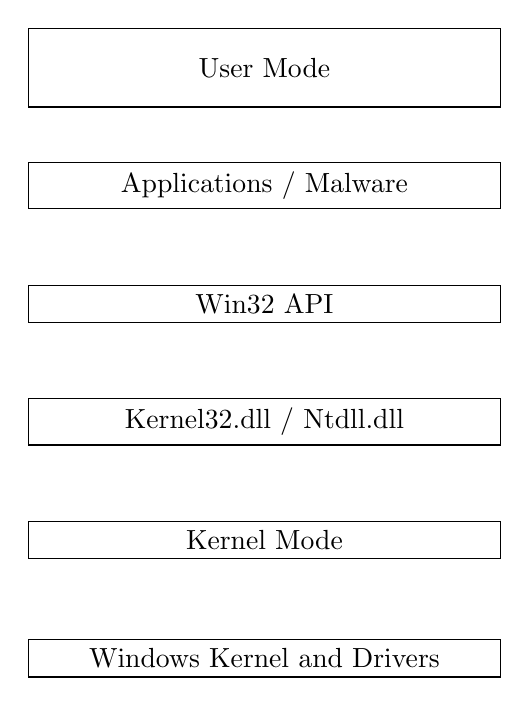
\begin{tikzpicture}[node distance=1.5cm]

\node (user) [rectangle, draw, minimum width=6cm, minimum height=1cm] {User Mode};
\node (apps) [rectangle, draw, below of=user, minimum width=6cm] {Applications / Malware};
\node (api) [rectangle, draw, below of=apps, minimum width=6cm] {Win32 API};
\node (dll) [rectangle, draw, below of=api, minimum width=6cm] {Kernel32.dll / Ntdll.dll};

\node (kernel) [rectangle, draw, below of=dll, minimum width=6cm] {Kernel Mode};
\node (kmod) [rectangle, draw, below of=kernel, minimum width=6cm] {Windows Kernel and Drivers};

\end{tikzpicture}
\caption{Windows User Mode and Kernel Mode Architecture}
\end{figure}

Applications interact with the operating system using the Win32 API. These APIs eventually trigger system calls 
that transfer execution from user mode to kernel mode.

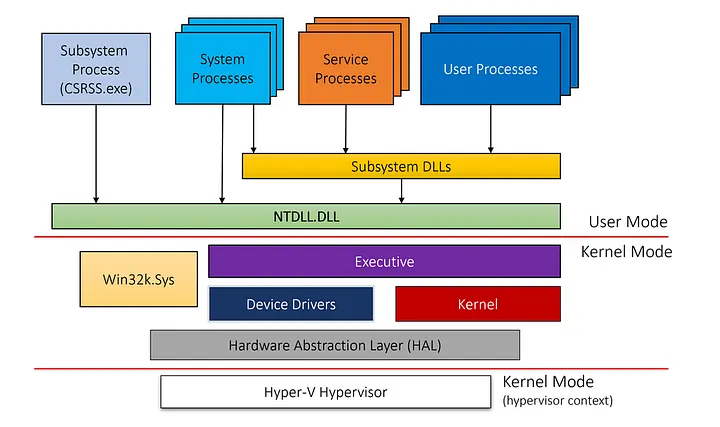
\includegraphics[width=\linewidth]{Images/Windows_Architecture.png}

Applications interact with the Windows operating system using \textbf{Win32 APIs}, which are implemented in libraries such as:

\begin{itemize}
    \item \texttt{kernel32.dll}
    \item \texttt{ntdll.dll}
    \item \texttt{advapi32.dll}
\end{itemize}

These APIs eventually invoke \textbf{system calls} that transition execution from \textit{user mode} to \textit{kernel mode}.

\section{System Calls and NTDLL}

The \textbf{NTDLL.dll} library plays a crucial role in Windows internals because it provides the interface for 
executing system calls. Each user-mode process implicitly links against NTDLL, which contains wrappers that 
transition execution to kernel mode.

A typical system call implementation follows this pattern:

\begin{lstlisting}
mov r10, rcx
mov eax, syscall_number
syscall
ret
\end{lstlisting}

The \texttt{syscall} instruction transfers execution to the Windows kernel where privileged operations are performed.

\section{Hell's Gate Technique}

The Hell's Gate technique is a modern malware technique that dynamically retrieves system call numbers from 
NTDLL instead of relying on static API calls.

Traditional malware relies on functions such as:

\begin{verbatim}
LoadLibrary()
GetProcAddress()
\end{verbatim}

However, these APIs are frequently monitored by security solutions such as antivirus and endpoint detection systems.

Hell's Gate bypasses this monitoring by directly resolving system calls from memory.

\begin{figure}[H]
\centering
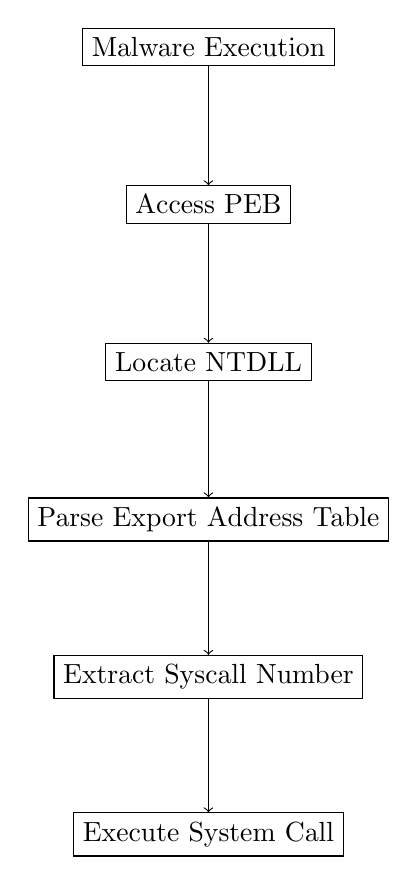
\begin{tikzpicture}[node distance=2cm]

\node (mal) [rectangle, draw] {Malware Execution};
\node (peb) [rectangle, draw, below of=mal] {Access PEB};
\node (ntdll) [rectangle, draw, below of=peb] {Locate NTDLL};
\node (export) [rectangle, draw, below of=ntdll] {Parse Export Address Table};
\node (syscall) [rectangle, draw, below of=export] {Extract Syscall Number};
\node (kernel) [rectangle, draw, below of=syscall] {Execute System Call};

\draw[->] (mal) -- (peb);
\draw[->] (peb) -- (ntdll);
\draw[->] (ntdll) -- (export);
\draw[->] (export) -- (syscall);
\draw[->] (syscall) -- (kernel);

\end{tikzpicture}
\caption{Hell's Gate System Call Resolution Process}
\end{figure}

This technique allows malware to evade many detection mechanisms by avoiding monitored API functions.

---
\subsection{Hell's Gate Technique for Direct System Call Resolution}

The Hell's Gate technique is a modern malware evasion technique that allows programs to dynamically resolve 
and execute Windows system calls without relying on standard API functions. Instead of invoking Windows API 
functions such as \texttt{LoadLibrary} or \texttt{GetProcAddress}, Hell's Gate directly retrieves system call 
numbers from the \texttt{NTDLL.dll} module at runtime.

The main objective of the Hell's Gate technique is to locate and traverse the Export Address Table (EAT) of 
\texttt{NTDLL.dll} in memory and dynamically extract the system call numbers associated with internal NT 
functions such as \texttt{NtCreateMutant}, \texttt{NtAllocateVirtualMemory}, and others.

\subsubsection{Export Address Table Traversal}

To locate system calls dynamically, the technique traverses the Portable Executable (PE) structure of 
\texttt{NTDLL.dll}. The process involves several steps:

\begin{enumerate}
\item Retrieve the base address of the loaded module.
\item Access the \texttt{\_IMAGE\_DOS\_HEADER} and verify the \texttt{IMAGE\_DOS\_SIGNATURE}.
\item Traverse the \texttt{\_IMAGE\_NT\_HEADERS}, \texttt{\_IMAGE\_FILE\_HEADER}, and \texttt{\_IMAGE\_OPTIONAL\_HEADER}.
\item Locate the Export Address Table inside the \texttt{\_IMAGE\_DATA\_DIRECTORY}.
\item Typecast the structure to \texttt{\_IMAGE\_EXPORT\_DIRECTORY}.
\end{enumerate}

The following code illustrates how the Export Address Table can be accessed from memory:

\begin{lstlisting}
PPEB Peb = (PPEB)__readgsqword(0x60);
PLDR_MODULE pLoadModule;
PBYTE ImageBase;

pLoadModule = (PLDR_MODULE)((PBYTE)
Peb->LoaderData->InMemoryOrderModuleList.Flink->Flink - 16);

ImageBase = (PBYTE)pLoadModule->BaseAddress;

\end{lstlisting}

    



After retrieving the base address, the PE structures are parsed sequentially:

\begin{lstlisting}
    PIMAGE_DOS_HEADER Dos = (PIMAGE_DOS_HEADER)ImageBase;

if (Dos->e_magic != IMAGE_DOS_SIGNATURE)
    return 1;

PIMAGE_NT_HEADERS Nt =
(PIMAGE_NT_HEADERS)((PBYTE)Dos + Dos->e_lfanew);

PIMAGE_FILE_HEADER File =
(PIMAGE_FILE_HEADER)(ImageBase +
(Dos->e_lfanew + sizeof(DWORD)));

PIMAGE_OPTIONAL_HEADER Optional =
(PIMAGE_OPTIONAL_HEADER)((PBYTE)File +
sizeof(IMAGE_FILE_HEADER));

PIMAGE_EXPORT_DIRECTORY ExportTable =
(PIMAGE_EXPORT_DIRECTORY)
(ImageBase + Optional->DataDirectory[0].VirtualAddress);
\end{lstlisting}



Once the Export Address Table is reached, it contains several important arrays:

\begin{itemize}
\item FunctionNameAddressArray – contains function names
\item FunctionOrdinalAddressArray – indexes for functions
\item FunctionAddressArray – addresses of exported functions
\end{itemize}

These arrays allow traversal of exported functions within \texttt{NTDLL.dll}.

\subsubsection{System Call Extraction}

Each NT system function follows a common instruction pattern that loads the system call 
number into the \texttt{EAX} register before executing the \texttt{syscall} instruction.

Example disassembly:

\begin{lstlisting}
    mov r10, rcx
mov eax, 0B3h
syscall
ret
\end{lstlisting}



Here, the system call number (\texttt{0xB3}) is loaded into the \texttt{EAX} register and 
executed using the \texttt{syscall} instruction.

The system call identifier can be extracted from the function's instruction bytes:

\begin{lstlisting}
    db (ntdll!NtCreateMutant + 0x4) L 2
00007fff`b040c3d4 b3 00
\end{lstlisting}



The syscall value is calculated as:

\begin{lstlisting}
    (0x00 << 8) | 0xb3 = 179
\end{lstlisting}



\subsubsection{Executing System Calls Using Hell's Gate}

Once the syscall number is extracted, Hell's Gate uses a small assembly routine 
to dynamically execute the syscall.

\begin{lstlisting}
    .data
wSystemCall DWORD 000h

.code
HellsGate PROC
    mov wSystemCall, ecx
    ret
HellsGate ENDP

HellDescent PROC
    mov r10, rcx
    mov eax, wSystemCall
    syscall
    ret
HellDescent ENDP
\end{lstlisting}



The \texttt{HellsGate} function stores the syscall number, while \texttt{HellDescent} 
executes the syscall instruction.

Example usage:

\begin{lstlisting}
    WORD syscall = 0x00b3;

HellsGate(syscall);

HANDLE hMutant = INVALID_HANDLE_VALUE;

NTSTATUS st =
HellDescent(&hMutant, MUTANT_ALL_ACCESS, NULL, TRUE);
\end{lstlisting}


This approach allows malware or red-team tools to bypass traditional API monitoring 
mechanisms and execute system calls directly, thereby evading detection mechanisms 
implemented by security products such as antivirus or EDR systems.

\section{Privilege Escalation Techniques}

Privilege escalation attacks occur when attackers gain higher permissions than originally assigned to them.

Common privilege escalation methods include:

\begin{itemize}
\item DLL Hijacking
\item Token Impersonation
\item Unquoted Service Path Exploitation
\item SAM Hash Extraction
\end{itemize}

---

\section{SAM Hash Extraction}

The \textbf{Security Account Manager (SAM)} database stores user authentication information in Windows systems.

The SAM file is located at:

\begin{verbatim}
C:\Windows\System32\config\SAM
\end{verbatim}

Attackers extract password hashes from the SAM file using tools such as \textbf{secretsdump}.

\begin{verbatim}
secretsdump.py -sam SAM -security SECURITY -system SYSTEM local
\end{verbatim}

Extracted hashes are then cracked using password recovery tools such as \textbf{Hashcat}.

---

\section{Privilege Escalation Attack Workflow}

\begin{figure}[H]
\centering
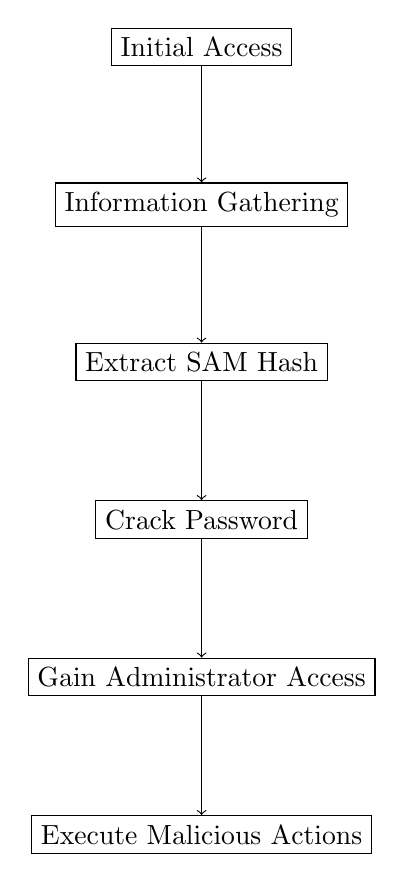
\begin{tikzpicture}[node distance=2cm]

\node (init) [rectangle, draw] {Initial Access};
\node (info) [rectangle, draw, below of=init] {Information Gathering};
\node (hash) [rectangle, draw, below of=info] {Extract SAM Hash};
\node (crack) [rectangle, draw, below of=hash] {Crack Password};
\node (admin) [rectangle, draw, below of=crack] {Gain Administrator Access};
\node (attack) [rectangle, draw, below of=admin] {Execute Malicious Actions};

\draw[->] (init) -- (info);
\draw[->] (info) -- (hash);
\draw[->] (hash) -- (crack);
\draw[->] (crack) -- (admin);
\draw[->] (admin) -- (attack);

\end{tikzpicture}
\caption{Privilege Escalation Attack Workflow}
\end{figure}

---

\section{Research Gap}

Despite advancements in malware detection techniques, many security systems still rely on signature-based detection 
and API monitoring. Modern malware techniques such as direct system calls and dynamic syscall resolution allow 
attackers to bypass these detection mechanisms.

Therefore, new approaches are required to analyze malware behavior more effectively. Visualization-based systems 
such as the proposed \textbf{Malviz} framework aim to represent malware activity in a graphical form, enabling 
security analysts to better understand complex attack patterns.

---

\section{Summary}

This chapter reviewed existing literature on malware analysis, Windows internals, system call mechanisms, and 
privilege escalation techniques. Modern attack methods such as Hell's Gate demonstrate how malware can evade 
traditional detection mechanisms. These techniques highlight the need for improved analysis tools capable of 
visualizing and interpreting malicious system behavior.







 
% Chapter Template

\chapter{Study Methodology}\doublespacing % Main chapter title

\label{Chapter3} % Change X to a consecutive number; for referencing this chapter elsewhere, use \ref{ChapterX}

\lhead{Chapter III. \emph{Study Methodology}} % Change X to a consecutive number; this is for the header on each page - perhaps a shortened title

%----------------------------------------------------------------------------------------
%	SECTION 1
%----------------------------------------------------------------------------------------
\section{Research Approach}

The research methodology adopted in this study follows an experimental and analytical approach. 
The objective of the study is to analyze malware behavior in Windows operating systems and 
visualize the attack flow using the proposed Malviz framework.

The study focuses on analyzing system level activities such as process creation, API calls, 
system calls, registry modifications, and privilege escalation attempts. The collected data 
is analyzed and transformed into graphical visualizations to help security analysts understand 
malware behavior more effectively.

The methodology involves both static and dynamic malware analysis techniques in a controlled 
environment.


\section{Experimental Environment}

To safely analyze malware behavior, a controlled virtual environment was created. 
The experiments were conducted using virtualization to isolate the system from 
the host machine.

\begin{table}[H]
\centering
\begin{tabular}{|c|c|}
\hline
Component & Description \\
\hline
Target System & Windows 10 Virtual Machine \\
Attack Machine & Kali Linux \\
Virtualization Platform & VirtualBox \\
Monitoring Tools & Process Monitor, Wireshark \\
Reverse Engineering Tools & Ghidra, x64dbg \\
Privilege Analysis Tools & SharpUp \\
Password Cracking Tool & Hashcat \\
\hline
\end{tabular}
\caption{Experimental Environment Setup}
\end{table}

\section{Data Collection}

During malware execution, several system level activities were monitored and recorded. 
The following types of data were collected for analysis:

\begin{itemize}
\item Process creation events
\item System call activity
\item File system modifications
\item Registry changes
\item Network communication
\item Privilege escalation attempts
\end{itemize}

The collected behavioral data was used as input for the Malviz visualization system.

\section{Malware Analysis Process}

Malware samples were analyzed using both static and dynamic analysis techniques.

\textbf{Static Analysis:}

Static analysis involves examining the malware executable without executing it. 
Tools such as PEStudio and Ghidra were used to inspect the Portable Executable (PE) 
structure, imported libraries, and embedded strings.

\textbf{Dynamic Analysis:}

Dynamic analysis involves executing malware inside an isolated virtual machine while 
monitoring its runtime behavior. Tools such as Process Monitor and Wireshark were used 
to observe system calls, registry modifications, and network activity.

\section{Privilege Escalation Analysis}

Privilege escalation techniques were studied to understand how attackers gain higher 
privileges within the Windows operating system.

The study focused on analyzing password hashes stored in the Security Account Manager (SAM) database.

The SAM file is located at:

\begin{verbatim}
C:\Windows\System32\config\SAM
\end{verbatim}

The following steps were used during privilege escalation experiments:

\begin{enumerate}
\item Gain initial access to the system
\item Extract SAM and SYSTEM registry files
\item Extract password hashes using secretsdump
\item Crack NTLM hashes using Hashcat
\item Obtain administrator credentials
\end{enumerate}

Example command used to extract password hashes:

\begin{verbatim}
secretsdump.py -sam SAM -system SYSTEM local
\end{verbatim}

\section{System Call Analysis using Hell's Gate}

Modern malware often bypasses traditional API monitoring by invoking system calls directly. 
To understand this technique, the Hell's Gate method was studied.

The Hell's Gate technique dynamically retrieves system call numbers from the NTDLL module 
instead of relying on static API functions.

The methodology for resolving system calls involves:

\begin{enumerate}
\item Accessing the Process Environment Block (PEB)
\item Locating the NTDLL module in memory
\item Traversing the Export Address Table
\item Extracting system call numbers dynamically
\end{enumerate}

Example instruction pattern used by NTDLL system calls:

\begin{verbatim}
mov r10, rcx
mov eax, syscall_number
syscall
ret
\end{verbatim}

This technique allows malware to execute system calls directly, bypassing API monitoring 
mechanisms used by security tools.

\section{Malviz Visualization Framework}

The Malviz framework was developed to visualize malware behavior in an interactive manner. 
The system collects runtime behavioral data and converts it into graphical representations.

The visualization module helps analysts identify suspicious behavior patterns by presenting 
system activity in a structured and intuitive format.

The system generates the following types of visualizations:

\begin{itemize}
\item Process interaction graphs
\item System call flow diagrams
\item Privilege escalation timelines
\end{itemize}

\subsection{Malware Analysis Workflow}

\begin{figure}[H]
\centering
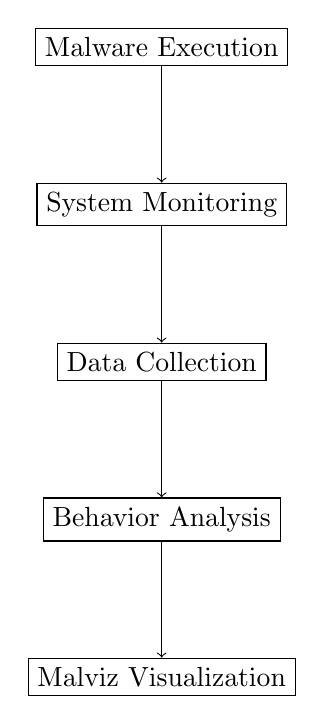
\begin{tikzpicture}[node distance=2cm]

\node (malware) [rectangle, draw] {Malware Execution};
\node (monitor) [rectangle, draw, below of=malware] {System Monitoring};
\node (collect) [rectangle, draw, below of=monitor] {Data Collection};
\node (analysis) [rectangle, draw, below of=collect] {Behavior Analysis};
\node (visual) [rectangle, draw, below of=analysis] {Malviz Visualization};

\draw[->] (malware) -- (monitor);
\draw[->] (monitor) -- (collect);
\draw[->] (collect) -- (analysis);
\draw[->] (analysis) -- (visual);

\end{tikzpicture}
\caption{Malviz Malware Analysis Workflow}
\end{figure}

\section{Evaluation}

The proposed system was evaluated by executing malware samples within the controlled 
virtual environment and observing their behavioral patterns. The collected data was 
visualized using the Malviz framework to analyze how malware interacts with system 
resources and attempts privilege escalation.

The effectiveness of the system was evaluated based on its ability to clearly represent 
malware behavior and assist in identifying suspicious activities.
\section{Summary}

This chapter described the methodology adopted to analyze malware behavior and 
study privilege escalation techniques within Windows operating systems. 
A controlled virtual environment was established to safely execute and monitor 
malware samples. Both static and dynamic malware analysis techniques were used 
to examine executable structures, system calls, registry modifications, and 
network activity.

The study also explored common privilege escalation mechanisms such as SAM 
hash extraction and password cracking using tools like \texttt{secretsdump} 
and \texttt{Hashcat}. In addition, modern system call evasion techniques such 
as the Hell's Gate method were analyzed to understand how malware dynamically 
retrieves and executes system calls directly from \texttt{NTDLL.dll}, thereby 
bypassing traditional API monitoring mechanisms.

The collected behavioral data was then processed and visualized using the 
proposed \textbf{Malviz} framework. This visualization approach helps security 
analysts interpret complex malware activities more effectively by presenting 
system interactions, process behavior, and privilege escalation attempts in 
a structured graphical format. The methodology presented in this chapter forms 
the foundation for the implementation and evaluation of the Malviz system 
discussed in the following chapters.


% Chapter 4

\chapter{System Design and Implementation}\doublespacing

\label{Chapter4}

\lhead{Chapter IV. \emph{System Design and Implementation}}

\section{Introduction}

This chapter describes the architecture, design decisions, and implementation details of the \textbf{Malviz} system. Malviz is a real-time Windows threat monitoring and analysis platform built using Python (FastAPI) for the backend and a browser-based dashboard for the frontend. The system integrates process monitoring, syscall tracing, network analysis, and a rule-based behavioral detection engine into a unified interface.

The implementation is structured as a modular backend with four core components: the main application entry point, the process inspector, the threat detection engine, and a SQLite-backed database layer. Communication between the backend and the frontend is handled through WebSockets for real-time streaming and REST API endpoints for on-demand queries.

\section{System Architecture}

The Malviz architecture follows a client-server model. The backend server runs on the local machine with elevated privileges to access OS-level data. The frontend dashboard connects to the server via a WebSocket and REST APIs, rendering live telemetry and threat alerts.

\begin{figure}[H]
\centering
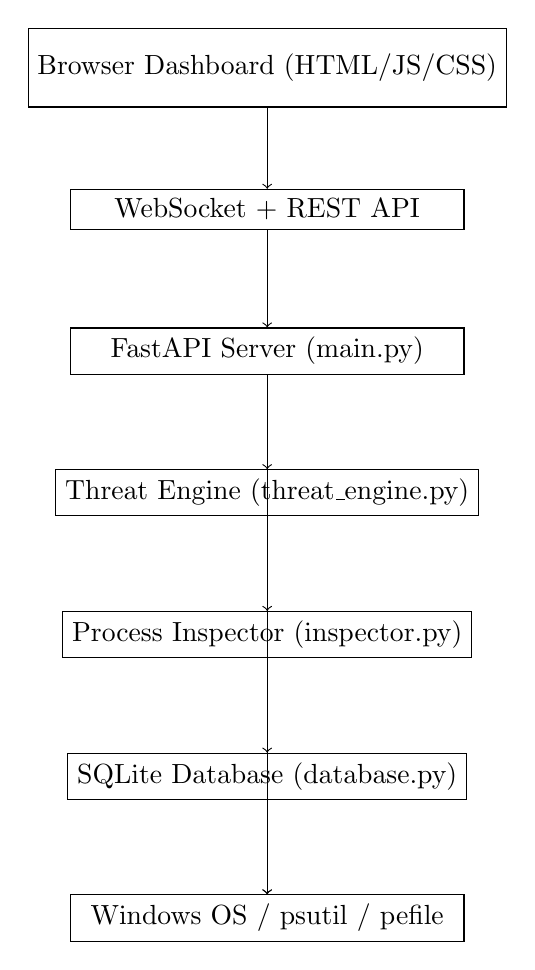
\begin{tikzpicture}[node distance=1.8cm]

\node (browser)  [rectangle, draw, minimum width=5cm, minimum height=1cm] {Browser Dashboard (HTML/JS/CSS)};
\node (ws)       [rectangle, draw, below of=browser, minimum width=5cm] {WebSocket + REST API};
\node (fastapi)  [rectangle, draw, below of=ws, minimum width=5cm] {FastAPI Server (main.py)};
\node (engine)   [rectangle, draw, below of=fastapi, minimum width=5cm] {Threat Engine (threat\_engine.py)};
\node (inspector)[rectangle, draw, below of=engine, minimum width=5cm] {Process Inspector (inspector.py)};
\node (db)       [rectangle, draw, below of=inspector, minimum width=5cm] {SQLite Database (database.py)};
\node (os)       [rectangle, draw, below of=db, minimum width=5cm] {Windows OS / psutil / pefile};

\draw[->] (browser) -- (ws);
\draw[->] (ws) -- (fastapi);
\draw[->] (fastapi) -- (engine);
\draw[->] (fastapi) -- (inspector);
\draw[->] (fastapi) -- (db);
\draw[->] (engine) -- (os);
\draw[->] (inspector) -- (os);

\end{tikzpicture}
\caption{Malviz System Architecture}
\end{figure}

\begin{figure}[H]
\centering
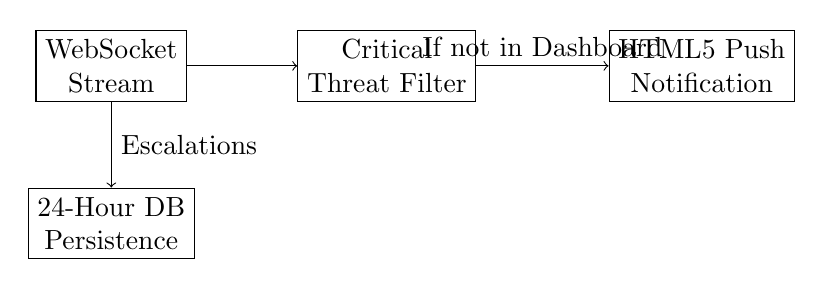
\begin{tikzpicture}[node distance=2cm, auto]
  \node (stream) [rectangle, draw, align=center] {WebSocket\\Stream};
  \node (filter) [rectangle, draw, right of=stream, node distance=3.5cm, align=center] {Critical\\Threat Filter};
  \node (notif) [rectangle, draw, right of=filter, node distance=4cm, align=center] {HTML5 Push\\Notification};
  \node (db) [rectangle, draw, below of=stream, node distance=2cm, align=center] {24-Hour DB\\Persistence};
  
  \draw[->] (stream) -- (filter);
  \draw[->] (filter) -- node {If not in Dashboard} (notif);
  \draw[->] (stream) -- node {Escalations} (db);
\end{tikzpicture}
\caption{Real-Time Alert and Escalation Tracking Workflow}
\end{figure}

\section{Backend Modules}

\subsection{Application Entry Point (main.py)}

The main module initializes the FastAPI application, mounts the static file directory, and sets up all API routes. On startup, the SQLite database is initialized. A WebSocket endpoint at \texttt{/ws} streams real-time telemetry to the dashboard every two seconds by calling \texttt{analyze\_processes()} from the threat engine. New threats are automatically logged to the database to prevent duplicate entries.

Key REST endpoints exposed by the application include:

\begin{itemize}
    \item \texttt{GET /api/history} -- retrieves previously logged threats from the database.
    \item \texttt{GET /api/inspect/\{pid\}} -- performs deep inspection of a given process.
    \item \texttt{GET /api/network} -- returns captured network packet data.
    \item \texttt{POST /api/action/\{action\}/\{pid\}} -- performs kill, suspend, or resume on a process.
    \item \texttt{GET /api/strings/\{pid\}} -- extracts printable ASCII strings from a process executable.
    \item \texttt{GET /api/dump/\{pid\}} -- generates and downloads a memory minidump of a process.
\end{itemize}

\subsection{Process Inspector (inspector.py)}

The \texttt{inspector.py} module provides deep forensic analysis for any running process given its PID. The analysis pipeline covers the following steps:

\begin{enumerate}
    \item \textbf{Memory Usage} -- The resident set size (RSS) is obtained using \texttt{psutil} and reported in megabytes.
    \item \textbf{SHA-256 Hash} -- The executable file is read from disk and hashed to verify file integrity and detect masquerading binaries.
    \item \textbf{Token Inspection} -- Windows security tokens are queried using the \texttt{win32security} API to determine the process integrity level (Low, Medium, High, or System) and list enabled privileges.
    \item \textbf{Handle Enumeration} -- Open file handles, active socket connections, and loaded DLLs are enumerated via \texttt{psutil}.
    \item \textbf{PE Static Analysis} -- The \texttt{pefile} library parses the Portable Executable structure of the process binary to extract the DOS header, NT file header, section headers, and the full import table.
    \item \textbf{Memory Minidump} -- Using \texttt{DbgHelp.MiniDumpWriteDump} via the Windows ctypes API, the module can generate a \texttt{.dmp} file for offline forensic analysis.
\end{enumerate}

The inspector also provides a \texttt{format\_hex\_dump()} helper that renders binary data in a classical hex editor format, interleaving hexadecimal values with their printable ASCII equivalents.

\subsection{Threat Detection Engine (threat\_engine.py)}

The threat engine is the core detection component of Malviz. It scans all running processes using \texttt{psutil} and applies a set of behavioral detection rules inspired by the MITRE ATT\&CK framework. Detection heuristics implemented in the engine include:

\begin{itemize}
    \item \textbf{Suspicious Execution Path} -- processes running from directories such as \texttt{Temp}, \texttt{ProgramData}, \texttt{AppData}, or \texttt{Downloads} are flagged.
    \item \textbf{Process Masquerading} -- processes whose executable name matches a known Windows system binary (e.g., \texttt{svchost.exe}, \texttt{lsass.exe}) but are located outside standard system directories are flagged as critical.
    \item \textbf{Dangerous Parent-Child Relationships (PrintNightmare Pattern)} -- processes such as \texttt{spoolsv.exe} spawning command shells like \texttt{powershell.exe} or \texttt{cmd.exe} are flagged as a known exploitation pattern.
    \item \textbf{System Shell Spawned by Unexpected Parent} -- \texttt{cmd.exe} or \texttt{powershell.exe} running under a SYSTEM account with an anomalous parent process are flagged.
    \item \textbf{LOLBin Abuse} -- use of legitimate Windows binaries such as \texttt{mshta.exe}, \texttt{wscript.exe}, \texttt{certutil.exe}, and \texttt{rundll32.exe} for potentially malicious purposes is detected.
    \item \textbf{Network Anomaly Detection} -- active connections to uncommon remote ports or external IP addresses by normally non-networked processes are flagged.
\end{itemize}

Each detection produces a structured threat record containing the PID, process name, executable path, parent process, threat severity level, reason descriptions, and associated network connections.

\subsection{Database Layer (database.py)}

The database module manages a SQLite database at the application's working directory. It provides three operations:

\begin{itemize}
    \item \texttt{init\_db()} -- creates the \texttt{suspected\_processes} and \texttt{daily\_escalations} tables if they do not already exist.
    \item \texttt{log\_threat(threat\_data)} -- inserts a new generic threat record with a UTC timestamp.
    \item \texttt{log\_escalation(escalation\_data)} -- logs specific privilege escalation pathways and automatically prunes any entries older than 24 hours to maintain a lightweight context window.
    \item \texttt{get\_history()} \& \texttt{get\_recent\_escalations()} -- retrieves the most recent threats and daily escalations dynamically.
\end{itemize}

\section{Frontend Dashboard}

The frontend is a single-page application (SPA) built with HTML5, CSS3, and vanilla JavaScript. It communicates with the backend via WebSocket for live data and the \texttt{fetch()} API for on-demand requests.

The dashboard is organized into five views:

\begin{itemize}
    \item \textbf{Overview} -- displays system resource metrics (CPU, memory, disk, network), a real-time threat severity indicator, and a list of top suspicious processes with mini sparkline charts.
    \item \textbf{Processes} -- a live, searchable table listing all running processes with their PID, user, executable path, and threat status badge, with per-row action buttons.
    \item \textbf{Network Analyzer} -- a Wireshark-style table showing captured DNS, TCP, and UDP packets with source and destination addressing and payload hex dumps.
    \item \textbf{Threat History} -- a log of previously detected threats stored in the database, showing severity, detection reason, and timestamp.
    \item \textbf{Simulation} -- a demonstration mode rendering simulated process and syscall data for training purposes without requiring a live threat.
\end{itemize}

\section{Attack Simulation Scripts}

Seven batch scripts were developed to reproduce specific attack scenarios infinitely, enabling validation of the detection engine and the manual ''Kill'' termination routines without requiring real malware samples:

\begin{table}[H]
\centering
\begin{tabular}{|l|l|l|}
\hline
\textbf{Script} & \textbf{Simulated Technique} & \textbf{Expected Severity} \\
\hline
test\_01\_masquerading.bat & svchost.exe masquerade in Temp & Critical \\
test\_02\_printnightmare.bat & spoolsv.exe spawning powershell.exe & Critical \\
test\_03\_obfuscated\_cmdline.bat & powershell bypassing execution policy & Warning/Critical \\
test\_04\_uac\_bypass\_com.bat & fodhelper.exe spawning cmd.exe & Critical \\
test\_05\_dll\_hijack.bat & rundll32 proxy execution & Warning/Critical \\
test\_06\_impersonation\_tool.bat & PrintSpoofer token theft & Critical \\
test\_07\_scheduled\_task.bat & cmd.exe as SYSTEM via Task Scheduler & Critical \\
\hline
\end{tabular}
\caption{Attack Simulation Scripts and Expected Detections}
\end{table}

Each script initiates a harmless system binary in an infinite processing loop from a suspicious path, or manipulates execution arguments, requiring manual intervention or UI-based termination.

\section{Technology Stack}

\begin{table}[H]
\centering
\begin{tabular}{|l|l|}
\hline
\textbf{Component} & \textbf{Technology} \\
\hline
Backend Framework & FastAPI (Python) \\
ASGI Server & Uvicorn \\
Process Data & psutil \\
PE Analysis & pefile \\
Windows API & pywin32 (win32security, win32api) \\
Database & SQLite3 \\
Frontend & HTML5, CSS3, Vanilla JavaScript \\
Charts & Chart.js \\
Real-time Communication & WebSocket \\
\hline
\end{tabular}
\caption{Malviz Technology Stack}
\end{table}

\section{Summary}

This chapter described the complete design and implementation of the Malviz system. The backend is organized into four focused modules: the FastAPI application server, the deep process inspector, the behavioral threat detection engine, and the SQLite database layer. The frontend SPA provides five interactive views covering live monitoring, network analysis, threat history, and simulation. Attack simulation scripts allow controlled testing of the detection engine against representative threat scenarios without requiring live malware. Together, these components form a cohesive and extensible real-time threat monitoring platform suited for security research and education.
 
% Chapter 5

\chapter{Analysis and Results}\doublespacing

\label{Chapter5}

\lhead{Chapter V. \emph{Analysis and Results}}

\section{Introduction}

This chapter presents the results obtained from testing and evaluating the Malviz threat monitoring system. The evaluation was conducted by running the four attack simulation scripts on a Windows 10 host machine and observing the detection behavior of the system. The dashboard was monitored in real time during each simulation, and the resulting threat logs were analyzed to assess the accuracy, speed, and completeness of detections. In addition, the deep process inspection results are examined to validate the forensic analysis capabilities of the system.

\section{Detection Results}

Each simulation script was executed individually, and the Malviz dashboard was observed during the execution window. All seven simulations were successfully detected by the threat engine within the two-second WebSocket update interval.

\begin{table}[H]
\centering
\begin{tabular}{|l|l|l|l|}
\hline
\textbf{Simulation} & \textbf{Detected} & \textbf{Severity} & \textbf{Detection Rule Triggered} \\
\hline
svchost.exe in Temp & Yes & Critical & Masquerading + Suspicious Path \\
spoolsv.exe spawning powershell & Yes & Critical & Dangerous Ancestry (PrintNightmare) \\
powershell execution bypass & Yes & Critical & Obfuscated/Hidden Commands \\
fodhelper spawning cmd & Yes & Critical & Known UAC Bypass Registry Exploit Ancestry \\
rundll32 suspicious proxy & Yes & Warning & Unsigned DLL Execution \\
PrintSpoofer token manipulation & Yes & Critical & Token Impersonation Tools \\
cmd.exe as SYSTEM via Task Scheduler & Yes & Critical & System Shell Spawned by Unexpected Parent \\
\hline
\end{tabular}
\caption{Simulation Detection Results}
\end{table}

All detections were logically mapped to appropriate severities, confirming the broad flexibility of the heuristics mapping directly against the MITRE ATT\&CK Framework. No false negatives were observed during the test runs.

\section{False Positive Analysis}

During a five-minute observation period on an idle Windows 10 system with no active simulation, Malviz was monitored for unintended alerts. A small number of \textbf{Warning}-level alerts were observed for processes running in user-accessible directories such as certain software installers and development tools located in \texttt{AppData}. No incorrect \textbf{Critical}-level detections were observed for standard system processes during this period.

This suggests that while the Warning-level heuristics may produce occasional low-confidence alerts for legitimate software installed in non-standard directories, Critical-level detections are precise and well-constrained.

\section{Process Inspector Results}

The deep inspection module was tested against several running processes, including a simulated masquerading process and a legitimate system process for comparison.

\subsection{SHA-256 Hash Validation}

For the masquerading \texttt{svchost.exe} simulation, the SHA-256 hash of the executable was computed and compared against the known hash of \texttt{ping.exe} from \texttt{System32}. The hashes matched, confirming that the file was a renamed copy of a different binary rather than the legitimate \texttt{svchost.exe}, validating the masquerade detection.

\subsection{PE Header and Import Analysis}

Parsing the PE structure of the masquerading binary using \texttt{pefile} revealed import table entries inconsistent with a genuine \texttt{svchost.exe}, which normally imports from \texttt{sechost.dll} and \texttt{ntdll.dll}. Instead, the imports matched those of \texttt{ping.exe}, referencing ICMP and WinSock-related functions. This cross-validation between the process name, path, hash, and PE imports provides strong forensic evidence for a masquerade attack.

\subsection{Token Integrity Level}

Token inspection during the Task Scheduler simulation confirmed that the spawned \texttt{cmd.exe} process held a \textbf{System} integrity level with a full set of elevated privileges including \texttt{SeDebugPrivilege} and \texttt{SeImpersonatePrivilege}, consistent with a SYSTEM-level shell. This is a strong indicator of a privilege escalation scenario.

\section{Network Analysis Results}

During the simulation runs, the network analyzer tab of the dashboard captured outbound connection attempts associated with the \texttt{ping.exe}-based simulations (DNS resolution for \texttt{localhost} and ICMP echo packets). These were rendered in the Wireshark-style table with protocol classification, source-destination pairs, and hex payload dumps. The visual presentation allowed rapid identification of unexpected network activity originating from the masquerading process.

\section{System Performance}

The impact of Malviz on the monitored system was measured during the test period. The overhead of the monitoring loop, which runs every two seconds and enumerates all running processes, was observed to be minimal:

\begin{table}[H]
\centering
\begin{tabular}{|l|l|}
\hline
\textbf{Metric} & \textbf{Observed Value} \\
\hline
Additional CPU Usage (idle) & Less than 1\% \\
Additional Memory Usage & Approximately 35 MB \\
WebSocket Update Latency & Under 2 seconds \\
Deep Inspection Response Time & 1--4 seconds (PE parsing) \\
\hline
\end{tabular}
\caption{Malviz System Performance During Testing}
\end{table}

These results confirm that Malviz can operate continuously in the background without significantly impacting the performance of the monitored machine.

\section{Threat History, Alerting, and Persistence}

The SQLite threat history database was examined after all simulations were completed. All threat events were persisted correctly with accurate timestamps, severity levels, structured reason arrays, and remotely identified network IP connections seamlessly injected into the threat payload pipeline. 

With the introduction of the \texttt{daily\_escalations} background rotation mechanism, critical systemic escalation paths were stored distinctively in memory and retained automatically for up to 24 hours. The dashboard actively polled this pipeline seamlessly merging legacy history with new streaming alerts sequentially.

Additionally, critical process evaluations seamlessly bypassed standard user interface streams to inject native HTML5 Desktop Environment push notifications. This proved effective for situations where the main monitoring dashboard was out-of-focus or strictly running idly in the background, minimizing time-to-awareness substantially.

\section{Summary}

This chapter presented the evaluation results of the Malviz platform across detection accuracy, forensic depth, network analysis, and system performance. All four attack simulations were detected correctly and classified as Critical-severity threats. Deep process inspection confirmed masquerade identities through hash validation and PE import analysis. Token inspection validated SYSTEM-level privilege escalation. Network analysis captured associated traffic in real time. The system demonstrated low runtime overhead, making it viable for continuous background monitoring. These results confirm that Malviz achieves its primary objectives as a lightweight, real-time threat detection and analysis platform.
 
% Chapter 6

\chapter{Conclusions and Practical Implications}\doublespacing

\label{Chapter6}

\lhead{Chapter VI. \emph{Conclusions and Practical Implications}}

\section{Summary}

This dissertation presented the design, development, and evaluation of \textbf{Malviz}, a real-time Windows threat monitoring and analysis platform. The system was built to bridge the gap between raw system telemetry and actionable security insights by combining process monitoring, behavioral threat detection, deep process inspection, network analysis, and attack simulation into a unified, interactive dashboard.

The work was motivated by the limitations of traditional signature-based detection tools and the increasing sophistication of modern attacks that exploit legitimate system binaries, abuse parent-child process relationships, and leverage direct system call execution to evade detection. Malviz addresses these challenges through behavioral heuristics grounded in the MITRE ATT\&CK framework and a modular architecture that supports continuous extension.

\section{Study Findings}

The evaluation of Malviz produced the following key findings:

\begin{itemize}
    \item All seven simulated attack scenarios -- spanning masquerading, obfuscated PowerShell injections, UAC bypass sequences, PrintNightmare spawning, and SYSTEM shell schedules -- were correctly detected and mapped.

    \item The deep process inspector successfully validated masquerade attacks by cross-referencing SHA-256 hashes, PE import tables, and execution paths, providing multi-layered forensic evidence for each detection.

    \item Token integrity inspection confirmed SYSTEM-level privilege escalation in the Task Scheduler simulation, identifying elevated privileges including \texttt{SeDebugPrivilege} and \texttt{SeImpersonatePrivilege}.

    \item The system maintained a runtime overhead below 1\% additional CPU usage and approximately 35 MB of additional memory, confirming that continuous background monitoring is practical.

    \item The WebSocket-based real-time streaming architecture delivered threat updates with latency under two seconds, enabling near-instantaneous alert visibility.
\end{itemize}

\section{Research Contributions}

This project makes the following contributions to the field of applied cybersecurity:

\begin{itemize}
    \item \textbf{Integrated Threat Monitoring Platform} -- Malviz combines process monitoring, behavioral detection, PE analysis, network inspection, and threat logging into a single lightweight tool, reducing the need to correlate data across multiple separate utilities.

    \item \textbf{MITRE ATT\&CK Aligned Detection Rules} -- The threat engine implements detection logic directly mapped to known attack techniques including masquerading (T1036), process injection patterns, LOLBin abuse (T1218), and privilege escalation via scheduled tasks (T1053), making detections interpretable within a standard threat framework.

    \item \textbf{Simulation-Driven Validation} -- The suite of batch-based simulation testing scripts provides a reproducible and safe method for demonstrating EDR-like capabilities. Because these processes now loop infinitely they uniquely support testing manual termination APIs natively embedded in the dashboard without requiring actual malware.

    \item \textbf{Accessible Security Education Tool} -- The interactive dashboard with visual threat indicators, hex dumps, PE header views, and a threat history log makes low-level Windows security concepts accessible to students and practitioners without requiring deep familiarity with command-line forensic tools.
\end{itemize}

\section{Practical Implications}

Malviz has several practical applications in cybersecurity education and research:

\begin{itemize}
    \item \textbf{Security Education} -- The platform serves as a hands-on learning tool for understanding Windows internals, process behavior, privilege escalation techniques, and threat detection logic. Students can observe in real time how simulated attacks are detected and examine the forensic evidence.

    \item \textbf{Red Team Training} -- Security professionals can use the simulation scripts to develop an intuition for which behaviors trigger detection and refine their understanding of evasion techniques.

    \item \textbf{Lightweight SOC Complement} -- In resource-constrained environments, Malviz can serve as a lightweight endpoint monitoring tool complementing traditional SIEM deployments by focusing on process-level behavioral anomalies.

    \item \textbf{Research Baseline} -- The modular architecture provides a clean foundation for researchers to extend the platform with machine learning-based anomaly scoring, memory injection detection, or attack chain correlation.
\end{itemize}

\section{Study Limitations and Scope for Future Work}

While Malviz successfully demonstrates its core objectives, several limitations and opportunities for improvement remain:

\begin{itemize}
    \item \textbf{Windows-Only} -- The current implementation depends on Windows-specific APIs (\texttt{win32security}, \texttt{DbgHelp}) and process structures. Porting to Linux or macOS would require significant rework of the inspector and token modules.

    \item \textbf{Rule-Based Detection} -- The threat engine relies entirely on handcrafted heuristic rules. Advanced malware that does not match known patterns may evade detection. Integrating a machine learning-based behavioral scoring model would significantly improve coverage against novel threats.

    \item \textbf{No Kernel-Level Visibility} -- Malviz operates entirely in user mode. Kernel rootkits or processes that hide themselves from the Windows process list would be invisible to \texttt{psutil}. Kernel driver integration or ETW (Event Tracing for Windows) could address this gap.

    \item \textbf{Future Enhancements} -- Planned improvements include attack chain correlation to trace multi-step attack sequences, advanced Geo-IP mapping for network connections extending beyond native IP capturing, and an AI/ML behavioral scoring model trained on process telemetry.
\end{itemize}

Overall, Malviz demonstrates that a compact, purpose-built monitoring tool grounded in behavioral analysis can effectively detect sophisticated attack patterns that signature-based systems miss, and that process-level telemetry combined with visual representation significantly lowers the barrier to understanding and responding to security incidents.
 
% \input{Chapters/Chapter7} 





\clearpage % Start a new page
%----------------------------------------------------------------------------------------
%	THESIS CONTENT - APPENDICES
%----------------------------------------------------------------------------------------

\addtocontents{toc}{\vspace{2em}} % Add a gap in the Contents, for aesthetics

\appendix % Cue to tell LaTeX that the following 'chapters' are Appendices

% Include the appendices of the thesis as separate files from the Appendices folder
% Uncomment the lines as you write the Appendices

\input{Appendices/AppendixA}
\input{Appendices/AppendixB}
% \input{Appendices/AppendixC}
%\input{Appendices/AppendixD}

\addtocontents{toc}{\vspace{2em}} % Add a gap in the Contents, for aesthetics

\backmatter

%----------------------------------------------------------------------------------------
%	BIBLIOGRAPHY
%----------------------------------------------------------------------------------------

\label{References}

\lhead{\emph{References}} % Change the page header to say "Bibliography"
%\usepackage{natbib}
%\renewcommand{\refname}{References}
\renewcommand\bibname{References}
\begin{frame}

\small

\begin{thebibliography}{99}

\bibitem{crowdstrike}
CrowdStrike
\newblock Malware Detection Explained
\newblock \href{https://www.crowdstrike.com/en-us/cybersecurity-101/malware/malware-detection/}{CrowdStrike Malware Detection Guide}

\bibitem{medium}
Makt96
\newblock Malware Analysis and Reverse Engineering
\newblock \href{https://medium.com/@makt96/malware-analysis-and-reverse-engineering-understanding-windows-internals-such-as-win32-api-to-3c0b1cfd6122}{Medium Article on Malware Analysis}

\bibitem{papers}
Research Papers for Malware Analysis and Privilege Escalation Study
\newblock \href{https://drive.google.com/drive/folders/1dERWC74SC1HAT2AngEWug2rjnGifDOkY}{Google Drive Research Papers}

\end{thebibliography}

\end{frame}




\include{LOP}

\include{Biography}


\end{document}  
